% $Id: template.tex 11 2007-04-03 22:25:53Z jpeltier $

\documentclass{vgtc}                          % final (conference style)
%\documentclass[review]{vgtc}                 % review
%\documentclass[widereview]{vgtc}             % wide-spaced review
%\documentclass[preprint]{vgtc}               % preprint
%\documentclass[electronic]{vgtc}             % electronic version

%% Uncomment one of the lines above depending on where your paper is
%% in the conference process. ``review'' and ``widereview'' are for review
%% submission, ``preprint'' is for pre-publication, and the final version
%% doesn't use a specific qualifier. Further, ``electronic'' includes
%% hyperreferences for more convenient online viewing.

%% Please use one of the ``review'' options in combination with the
%% assigned online id (see below) ONLY if your paper uses a double blind
%% review process. Some conferences, like IEEE Vis and InfoVis, have NOT
%% in the past.

%% Figures should be in CMYK or Grey scale format, otherwise, colour
%% shifting may occur during the printing process.

%% These few lines make a distinction between latex and pdflatex calls and they
%% bring in essential packages for graphics and font handling.
%% Note that due to the \DeclareGraphicsExtensions{} call it is no longer necessary
%% to provide the the path and extension of a graphics file:
%% \includegraphics{diamondrule} is completely sufficient.
%%
\ifpdf%                                % if we use pdflatex
  \pdfoutput=1\relax                   % create PDFs from pdfLaTeX
  \pdfcompresslevel=9                  % PDF Compression
  \pdfoptionpdfminorversion=7          % create PDF 1.7
  \ExecuteOptions{pdftex}
  \usepackage{graphicx}                % allow us to embed graphics files
  \DeclareGraphicsExtensions{.pdf,.png,.jpg,.jpeg} % for pdflatex we expect .pdf, .png, or .jpg files
\else%                                 % else we use pure latex
  \ExecuteOptions{dvips}
  \usepackage{graphicx}                % allow us to embed graphics files
  \DeclareGraphicsExtensions{.eps}     % for pure latex we expect eps files
\fi%

%% it is recomended to use ``\autoref{sec:bla}'' instead of ``Fig.~\ref{sec:bla}''
\graphicspath{{figures/}{pictures/}{images/}{./}} % where to search for the images

\usepackage{microtype}                 % use micro-typography (slightly more compact, better to read)
\PassOptionsToPackage{warn}{textcomp}  % to address font issues with \textrightarrow
\usepackage{textcomp}                  % use better special symbols
\usepackage{mathptmx}                  % use matching math font
\usepackage{times}                     % we use Times as the main font
\renewcommand*\ttdefault{txtt}         % a nicer typewriter font
\usepackage{cite}                      % needed to automatically sort the references
\usepackage{tabu}                      % only used for the table example
\usepackage{booktabs}                  % only used for the table example
%% We encourage the use of mathptmx for consistent usage of times font
%% throughout the proceedings. However, if you encounter conflicts
%% with other math-related packages, you may want to disable it.

\usepackage{xspace}

\usepackage{caption}
\captionsetup[table]{skip=10pt}
\usepackage{tabularx}
\usepackage{todonotes} %TODO: Remove after all TODO's are gone

%% ===================================== Commands
\newcommand{\code}[1]{\texttt{\small{#1}}}
\newcommand{\typevis}{{\sc TypeVis}\xspace}

%% If you are submitting a paper to a conference for review with a double
%% blind reviewing process, please replace the value ``0'' below with your
%% OnlineID. Otherwise, you may safely leave it at ``0''.
\onlineid{0}

%% declare the category of your paper, only shown in review mode
\vgtccategory{Research}

%% allow for this line if you want the electronic option to work properly
\vgtcinsertpkg

%% In preprint mode you may define your own headline.
%\preprinttext{To appear in an IEEE VGTC sponsored conference.}

\title{Type Visualization for R}

\author{Cameron Moy\thanks{camoy@ccs.neu.edu}
\and Julia Belyakova\thanks{belyakovay@ccs.neu.edu}}
\affiliation{\scriptsize Northeastern University}

\abstract{
  Data-driven approaches to programming language design are uncommon.
  Despite the availability of large code repositories, distilling useful
  information from programs remains difficult. Important dimensions,
  like run-time type data, are inscrutable without the appropriate tools.
  \typevis is an interactive visualization for exploring and analyzing
  type information from program execution traces---aiding
  user understanding of function type signatures across many executions.
  The system uses flows to intuitively represent categorical
  and numerical aspects of type signatures.
  Insights derived from our visualization are aimed at informing
  language design decisions---specifically of a new gradual type system
  currently being developed for the R programming language.
}

%% ACM Computing Classification System (CCS).
%% See <http://www.acm.org/about/class> for details.
%% We recommend the 2012 system <http://www.acm.org/about/class/class/2012>
%% For the 2012 system use the ``\CCScatTwelve'' which command takes four arguments.
%% The 1998 system <http://www.acm.org/about/class/class/2012> is still possible
%% For the 1998 system use the ``\CCScat'' which command takes four arguments.
%% In both cases the last two arguments (1998) or last three (2012) can be empty.

\CCScatlist{
  \CCScatTwelve{Human-centered computing}{Visualization}{Visualization systems and tools}{}
}

%% Copyright space is enabled by default as required by guidelines.
%% It is disabled by the 'review' option or via the following command:
% \nocopyrightspace

%%%%%%%%%%%%%%%%%%%%%%%%%%%%%%%%%%%%%%%%%%%%%%%%%%%%%%%%%%%%%%%%
%%%%%%%%%%%%%%%%%%%%%% START OF THE PAPER %%%%%%%%%%%%%%%%%%%%%%
%%%%%%%%%%%%%%%%%%%%%%%%%%%%%%%%%%%%%%%%%%%%%%%%%%%%%%%%%%%%%%%%%

\begin{document}

\firstsection{Introduction}

\maketitle

Programming languages commonly evolve by decree. Often, the language designer
decides that a new feature is necessary, or that a past feature was
ill-conceived. Thus, the language moves forward---
forcing its users to adapt to the changes.
Sometimes, these changes are the result of rigorous theory
or the product of community feedback. However, rarely is language design
informed by empirical data on how programs are \emph{actually
written} in practice. Why so?

%For a popular language, data collection is no challenge. Vast
Thanks to the prevalence of open source code, collecting data on
the usage of a popular programming language is feasible. Vast
quantities of publicly available code are hosted on repositories such as Github.
Furthermore, if there is concern about the quality of this data,
such as code duplication~\cite{lopes:2017},
code can be obtained from curated
language-specific package repositories like npm or CRAN.

To inform programming language design,
the collected data needs to be analyzed and interpreted.
Programs are complex and highly structured,
so simple semantically-ignorant metrics like ``lines of code'' carry little significance.
Therefore, researchers often employ static and dynamic analyses
to gather information about specific aspects of programs.
Even then, it may be difficult to make sense of the
results of these analyses,
especially if the data set is large.
%Rather, the difficulty lies with analyzing and interpreting the data
%at hand. Code is complex and highly structured. Simple

To analyze just one aspect of programming languages, \emph{type usage}, we
built \typevis, an interactive visualization of run-time type signatures.
%an interactive visualization of run-time types for the language R.
\typevis was created with the R programming language in mind,
and builds on a data set of execution traces
mined from the unit tests and vignettes
of the most widely used libraries in the R ecosystem.

The tool supports three broad tasks:
\begin{itemize}
  \setlength\itemsep{0em}
  \item filtering the data set down to an amenable subset;
  \item understanding the types of function arguments and returns;
  \item comparing type signatures across different functions.
\end{itemize}
%For filtering, \typevis uses the treemap idiom
%to convey the relative scale of different packages.
For exploring and filtering the data set,
\typevis relies on treemaps to represent R packages and functions,
with node size conveying relative popularity.
Additionaly, one can use a search box to directly filter
by function name.
Once a subset of one or more functions is selected,
their type signatures are encoded as flows over types,
where flow width is proportional to frequency.
These flows can be readily compared within the same function,
or between different functions.

\typevis can assist language designers during multiple phases of development.
For example, exploratory data analysis can identify unexpected edge cases,
or weed out language designs that are incompatible with existing programs.
\typevis was built in support of a new gradual type system for R,
whose adoption depends on integrating well with existing R code.
However, the visualization is not limited to R and can be used to
analyze type usage in any language where similar data is available.

Supplemental material, including the data and source code of
\typevis, is freely available: \todo{Fill with archival link}

%%

\section{Background and Prior Work}

R is a dynamically typed programming language widely used for
statistical computing. Unlike statically typed languages,
R programs do not contain type annotations
and never pass through a typechecker.
At run-time,
functions may be called with values of arbitrary type,
and may return values of arbitrary type.\footnote{
  We use the word ``type'' to mean what others may call a ``type tag.''
  This is a run-time concept---we do not assume a static type system
  because there is none. Indeed, the goal is to help design one!
  A ``type signature'' in this context is one particular configuration
  of argument and return types a function is called with at run-time.
}

Being a dynamically typed language most actively used in a single domain,
R is a good target for a gradual type system.
For statically typed languages, the type system is usually
an inseparable part of the language. Since they are designed
at the same time, the (static) type system precedes any code written
in the language.
A gradual type system, by contrast,
permits the integration of static and dynamic typing.
Such a type system is capable of seamlessly mixing typed and untyped regions of code.
Often, a gradual type system is designed atop
an existing dynamically typed language.
Since many R programs already exist,
a successful gradual type system must be capable of
typechecking idiomatic R code.
\typevis aims to clarify how existing R programs
use types to assist in this task.
While this is our motivation, the visualization's use
is not necessarily limited to this application.
Anyone who has an interest in how the real R programs use types
may find it useful.

We are not aware of any previous work that applies
visualization techniques for the purposes of programming language design.
However, there are existing publications on understanding
software systems through visualization.
Bohnet et al.~\cite{bohnet:2009} visualize massive program execution traces
to assist developers in code comprehension of large software systems.
Their tool applies pruning and summarization to reduce trace size.
The visualization focuses on call topology,
describing the structure of function invocations,
rather than types.
Telea et al.~\cite{telea:2009} also develop a methodology for displaying call structure.
However, they visualize call graphs of systems in their entirety,
rather than individual execution traces.
Our visualization can be thought of as a hybrid of the two,
investigating the system as a whole,
but doing so via execution traces.
In addition to standard call graphs,
LaToza and Myers~\cite{latoza:2011} adorn nodes and edges with extra information,
allowing the user gain further understanding of the system
under examination.
This includes indicating methods that come from the same class---a
basic form of type information.

%%

\bgroup
\def\arraystretch{1.75}
\begin{table*}
  \centering
  \begin{tabularx}{\linewidth}{c|c|c|X}
    Domain Goals & Search Task & Query Task & \multicolumn{1}{c}{Abstract Task Description} \\
    \hline
    Find Function & Locate & Identify & Finding a function is a location task, where the target function is known, but its location within the package hierarchy is not. Once the desired function is found, a user must be able to identify data of interest. \\

    Determine Types & Browse & Identify & Determining types is a browse task, where the target type signature is unknown, but the location of the function of interest is known. While browsing, a user must be able to identify the frequencies of particular type signatures.\\

    Compare Signatures & Lookup & Compare & Comparing type signatures is a lookup task where both target type signatures have already been located. A user must be able to discern how often a signature is used compared to another, both within a function and across different functions.\\
  \end{tabularx}
  \caption{Domain goals and their mid-level and low-level task abstractions.}
  \label{tab:tasks}
\end{table*}
\egroup

\section{Data and Collection}

\todo{Alexi's paper says 412, but I see more packages in our data.}

The data is provided by Alexi Turcotte:
it consists of traces from 412 packages
containing over $760,000$ lines of R code
and $534,000$ lines of native code.
All libraries were obtained from CRAN,
the most popular R code repository.
Packages hosted on CRAN must satisfy certain criteria
to ensure they are high quality.
Additionally, the subset of 412 packages chosen here
all had code coverage above 65\%.\todo{I don't understand what subset? Should we remove this line?}

Each execution trace was recorded by a dynamic analysis
running the test, example, and vignette code of each package.
A vignette is a form of documentation that weaves
together prose and executable code.
An execution trace is a list of ``raw'' function call signatures
containing, among other attributes, the function name
and type tags for each argument and return value.
For example, for the function call \code{!(FALSE)},
the recorded type signature would be \code{logical->logical},
meaning that function \code{!} took a logical value and returned a logical value.
The type tags are assigned by the dynamic analysis and
refine over actual type tags in R; for example, the analysis
assigns scalar tag \code{double} to a singleton vector of double values
because R does not have native support for scalars.
Our data set consists of a table of reduced execution traces:
because \typevis is designed for the analysis of types, not all information
in the traces is relevant.
%that have been processed to reduce some fields.
%Traces were generated via a dynamic analysis
%that instruments the R virtual machine with hooks
%that intercept the required data at run-time.

While \typevis has only been instantiated with
data from R execution traces, the architecture is not
limited to R.
Any dynamically typed language %with the right run-time
%hooks could generate data for the tool.
(or a statically typed language with run-time tag information)
could be instrumented to generate data for the tool.
As long as execution trace information adheres to
the same database schema, \typevis will
work properly without any modifications.

%%

\section{Task Abstraction}

We interviewed the primary researcher developing R's gradual type system
to inventory relevant domain-specific tasks.
Additionally, we sought feedback throughout the creation of \typevis
to ensure it was adequately satisfying requirements.
The domain-specific goals can be reduced to:

\begin{enumerate}
\item {\bf Find Function.} Quickly search for a particular function and identify basic information. This includes how often the function is called and which package contains it.
\item {\bf Determine Types.} Given a specific function, determine the argument and return types of the function. Additionally, identify the frequency of a type signature. A user should be able to infer, for example, if the function is polymorphic or if it's a predicate.
\item {\bf Compare Signatures.} Compare the occurrence of type signatures within a specific function, but also across many different ones. Users must be able to isolate individual signatures and see them in the context of other signatures and functions.
\end{enumerate}

These goals can be classified using an abstract task analysis framework.
See table~\ref{tab:tasks} for a categorization of these domain tasks
the mid-level and low-level abstract task taxonomy
established by Brehmer and Munzner~\cite{brehmer:2013}.

%%

\section{Design and Implementation}

\begin{figure*}
 \centering
 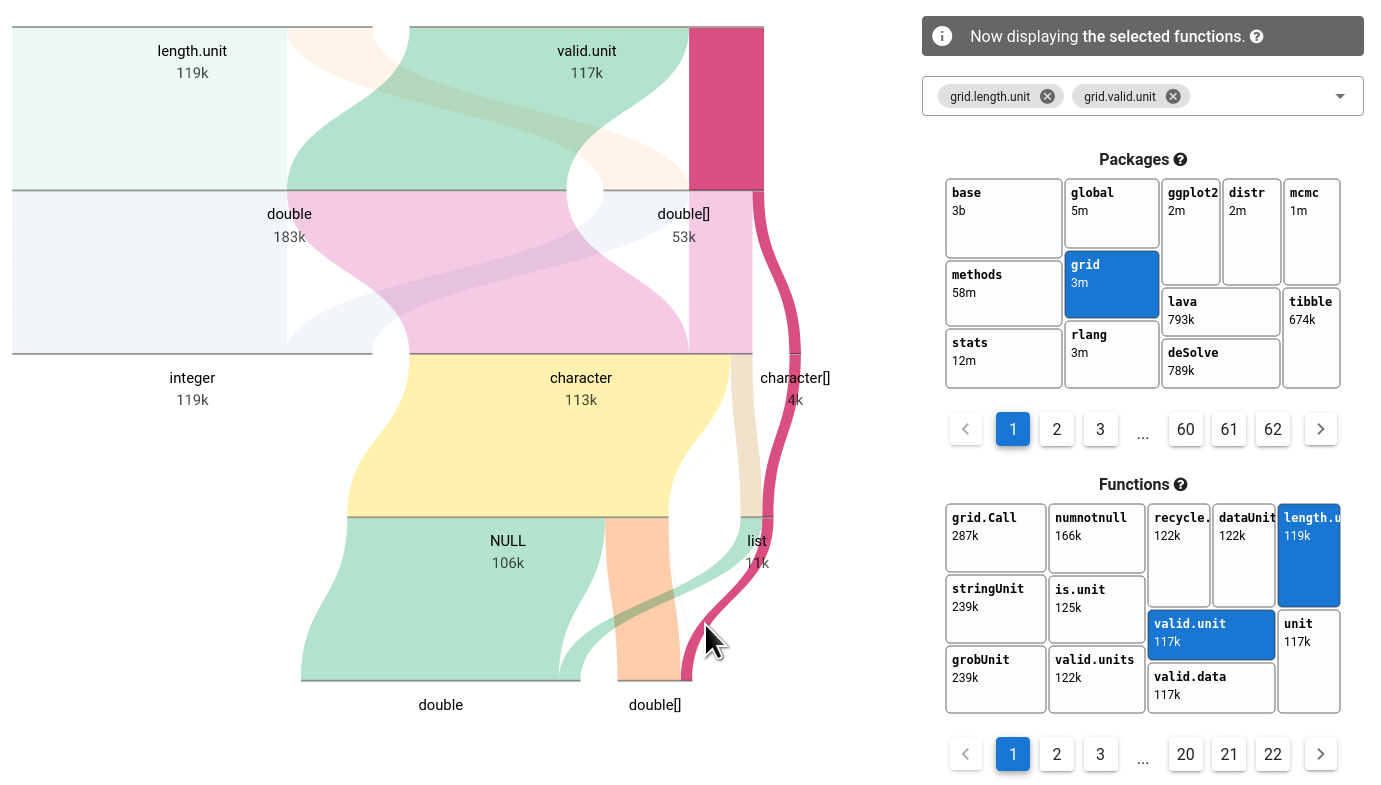
\includegraphics[width=\linewidth]{img/typevis.png}
 \caption{The main view of \typevis, with type flows on the left and the package hierarchy on the right. Here, the {\tt length.unit} and {\tt valid.unit} functions from the {\tt grid} package are both selected and displayed simultaneously.}
 \label{fig:typevis}
\end{figure*}

\typevis is an interactive web-based visualization
that permits real-time exploration,
even with large data sets.
The default data set contains over a million rows
based on the analysis of almost five hundred
different R packages.
Figure~\ref{fig:typevis} displays
the heart of \typevis
in its initial configuration.
Most aspects of the system can be tweaked
by a user if desired.

\subsection{Function Filtering}

The right-hand panel of figure~\ref{fig:typevis}
contains three elements: a search bar,
a package treemap,
and a function treemap.
All three are linked.
Selecting a package
in the top treemap will immediately narrow the
bottom view to only functions available in that package.
Additionally, entering a function name in the search
will select it in the function treemap.

These different components support different modes of search.
If a user has a specific function in mind,
the search bar supports autocomplete
that can quickly select a function among thousands.
However, if one wants to browse
all available functions and packages,
the treemap view is more applicable.
Nodes in the bottom treemap convey the log-scaled
frequency of function calls,
and correspondingly the top treemap
is scaled based on invocations
of functions defined in that package.
Log-scaling and pagination keep
elements of the treemap legible,
even if absolute size differences are significant.

Treemaps are often used for displaying hierarchical data~\cite{shneiderman:1992}.
Package systems in many languages,
like Java,
contain deeply nested namespace hierarchies.
This idiom is appropriate for navigation of such
hierarchies.
R packages are not structured deeply
so the treemaps in our data are only one
level deep.
However, if the data set was more deeply nested,
\typevis can be configured to
handle that.

If configured, \typevis allows for multiple function selection.
Both the {\tt length.unit} and {\tt valid.unit} functions
from the {\tt grid} package are selected in figure~\ref{fig:typevis}.
These functions are rendered simultaneously in the type flow
panel, allowing one to make comparisons between them.

\subsection{Types as Flows}

Prominently featured as the center visualization,
a parallel sets diagram encodes type signatures of the selected
functions as flows.
Parallel sets,
proposed by Kosara et al.~\cite{kosara:2006},
are ideally suited for type signatures.
Each data point is can be thought of as
a tuple $(f, \tau_1, \ldots, \tau_n)$
corresponding to the function name,
argument types,
and return type.
Every component is categorical,
and we are interested in visualizing frequencies of these points.
This is the exact use-case for parallel sets.

Flows begin at nodes labeling a function,
curve across each argument type in order,
and terminate at the return type.
Widths are proportional to how many times a function
is called with that signature during analysis.
Flow segments are filled with a hue-varying color scale,
based on the type where the segment ends.
Beneath each node label is an approximate count.
If the node represents a function, then the
number is how many times the function was invoked.
If the node represents a type, then the
number is how often a value of that type
at that argument position was recorded during analysis.

For example, in figure~\ref{fig:typevis},
the {\tt length.unit} function is called with
two different type signatures at run-time.
Most frequently, the function is used with the
signature {\tt double $\to$ integer},
but a substantial fraction of the time it is
used as {\tt double[] $\to$ integer}.
Here, {\tt double[]} stands for an array of
doubles with arbitrary dimension.

Interactivity significantly augments the
usability of the parallel sets visualization.
Hovering over a flow will highlight the
entire path of the flow
and will fade other functions
into the background.
When displaying many flows at the same time,
highlighting becomes especially critical
for user comprehension.
Additional quantitative information
about the flow is also supplied
while hovering.
Clicking a flow will focus on that function
only, filtering away all others.

Flow layout is a critical consideration
for a sufficiently legible visualization.
Figure~\ref{fig:decross} exemplifies what
happens if flow layout is not adequately handled.
The top layout was generated without any
flow decrossing algorithm,
while the bottom layout does
apply decrossing.
Even with highlighting,
the utility of the visualization is vastly
reduced without some decrossing effort.
To maintain real-time performance,
we use two different decrossing methods.
First, the system attempts to construct
a layout with the globally optimal
minimum amount of flow crossing by
solving a mixed-integer linear program.
Unfortunately, for even moderately
sized graphs this can take too long to compute.
Therefore, after about $1$ second
the optimal algorithm is terminated
if it has not finished, and a faster
algorithm that only locally minimizes crossing
between layers computes the layout.

\subsection{Technical Details}

Since the amount of data that a user may query is large,
the application consists of both a frontend and a backend.

On the frontend, state management, interactivity,
and DOM manipulation is all done within the Vue framework.
This is in contrast with many web-based visualizations
that use D3 for DOM manipulation.
We chose this setup because of the many different
individual components whose state must be kept
synchronized.
This includes not only the visualizations, but also
user interface elements like the autocomplete search bar.
In our experience, Vue's model of reactivity is
more successful at maintaining consistency across the
entire system than using D3 and vanilla JavaScript.
While \typevis does not use D3 for DOM manipulation,
it still does use D3 for other visualization-related
computations.

Our backend is a Node.js application that serves
JSON in a standard REST-style architecture.
Data is stored in a SQLite database that has been
indexed to achieve lookups as fast as possible.
To avoid excessive memory consumption and speed up computations,
clients query data from the server on an as-needed basis.
Thus, a stable network connection is required for
real-time interaction.

\begin{figure}[tb]
 \centering
 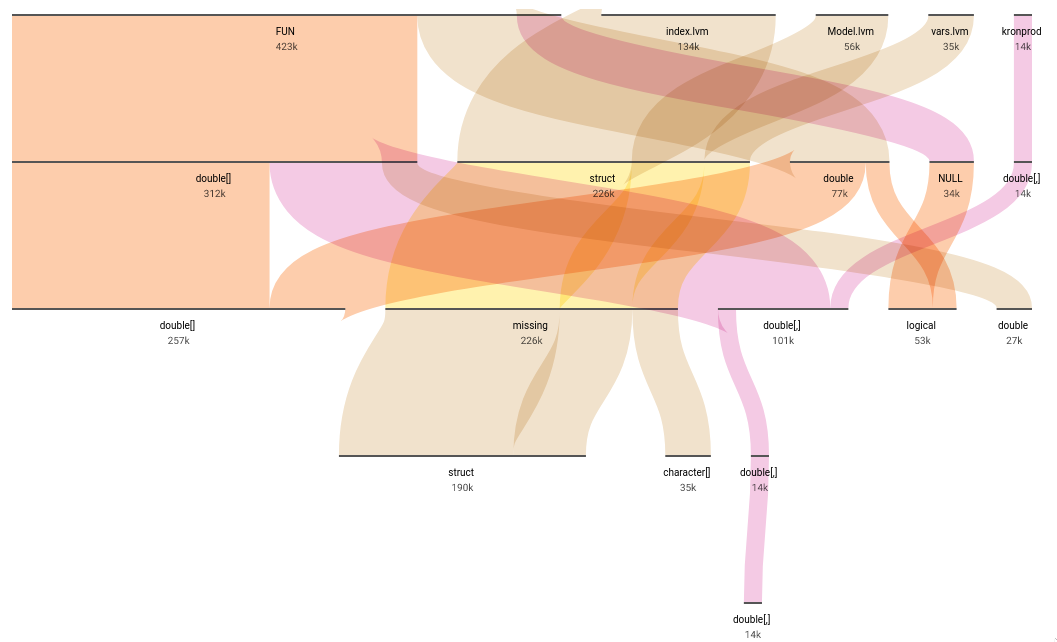
\includegraphics[width=\columnwidth]{img/no_decross.png}
 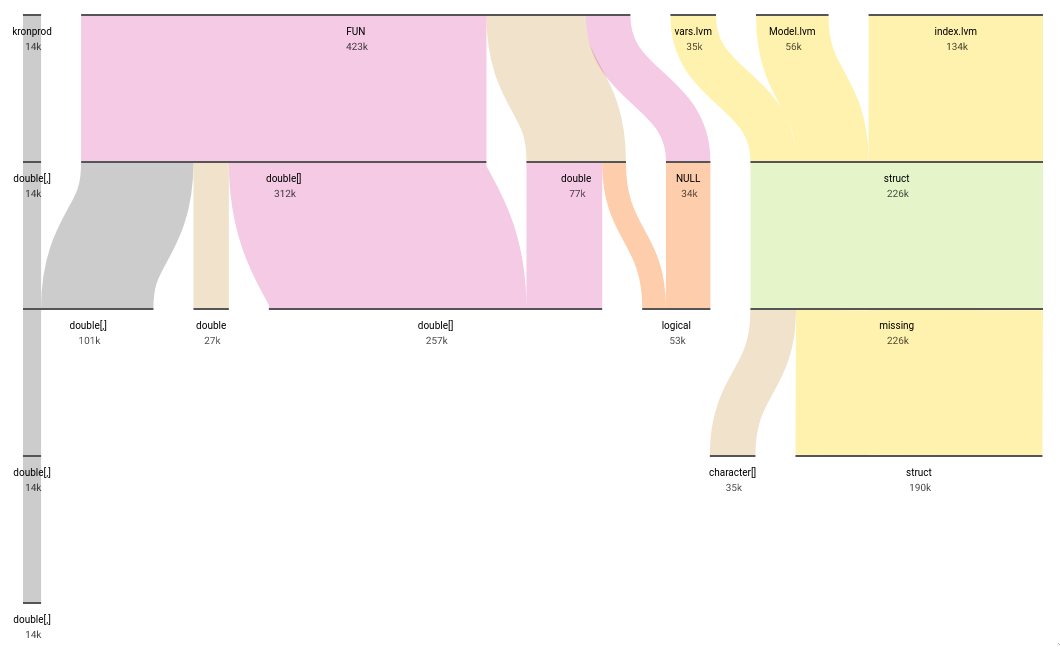
\includegraphics[width=\columnwidth]{img/decross.png}
 \caption{Comparison of type flows without decrossing (above) and with decrossing (below).}
 \label{fig:decross}
\end{figure}

%%

\section{Limitations and Future Work}

\typevis suffers from a number of shortcomings
and does not fully address the entire range of possible tasks
a language designer may need to perform.

In particular, R supports a wide range of data types
including types that contain dimensionality information.
For example, an R array may have type {\tt integer[3]}
indicating that it is an array of length $3$.
This will get compressed down into a single array
type labeled {\tt integer[]}.
Reducing the number of types can make the visualization
more understandable---at the expensive of losing some
precision in type information.
Ideally a user would be able to interactively tune
the level of type granularity based on their interest
in a specific property.
Such a feature would be especially helpful for R
since values can come attached with relevant additional
data such as the dynamic dispatch method
or user-specified metadata.

Filtering is an central mechanism in the system,
but it also comes at a cost.
If one has a specific function or several functions
in mind, then \typevis provides a useful
local view of that type information.
However, it does not support any kind of global
view of type information across a large amount of
functions. When the number of flows or nodes
becomes too great, the visualization will start
paginating, making comparisons over large amounts
of data impossible.
Aggregation and summarization would be key to
making a global view of the data feasible---that
remains future work.

%%

\section{Conclusion}

We have presented \typevis, an interactive visualization
of run-time type information for R.
It supports real-time exploration of a data set of
execution traces from a large corpus of R packages.
To narrow the data under consideration,
\typevis provides facilities for filtering
and searching.
Type signatures are represented as flows traversing across
each argument type and return type in sequence.
Flow widths are proportional to how often
that type signature was seen during the dynamic analysis.
Interactions provide additional details and
assist users in comprehension and navigation.

Our tool is aimed at elucidating how R programmers
use the language in practice.
Specifically, the data and visualization will be used to
inform the design of a gradual type system for R.
However, \typevis is not tied to the R ecosystem
and is suitable to use for any dynamically typed language
with a similar data set.
Additionally, the visualization could yield insights
useful for other purposes than gradual typing.

We hope that, in the future, programming language designers
will collect and use empirical data about how their languages
are used in practice.
Such data can be used to make informed decisions about
language design.
Visualization will be unavoidable in these scenarios
since semantically-meaning information about programs
is rich in structure.
Generic, canned visualizations will not be sufficient.
\typevis is just the first step in this direction.

\acknowledgments{
  The authors wish to thank the students of CS 7250 for useful design feedback,
  and contributors to all the open source projects that \typevis depends on.
  This work was supported in part by a Northeastern Graduate Fellowship.
}

\bibliographystyle{abbrv-doi}

\bibliography{main}
\end{document}
